
\subsection{Figuras e vídeos}

\begin{frame}
	
	\only<presentation>{\vspace*{-\bigskipamount}}%% Apresentação: espaçamento
	
	\begin{columns}[t]
		
		\column{0.5\textwidth-0.5\columnsep}
		
		A Figura~\ref{fig:campi-map}\footnote{Possui um código QR contendo um URL.} apresenta um mapa com a localização dos campi da UTFPR\@.
		
		\begin{figure}[!htb]
			\caption{Localização dos campi da UTFPR}%
			\label{fig:campi-map}
			\only<presentation>{\dimen1 = 40mm}%% Apresentação: tamanho de figura
			\only<article>{\dimen1 = 54mm}%% Artigo: tamanho de figura
			\savebox0{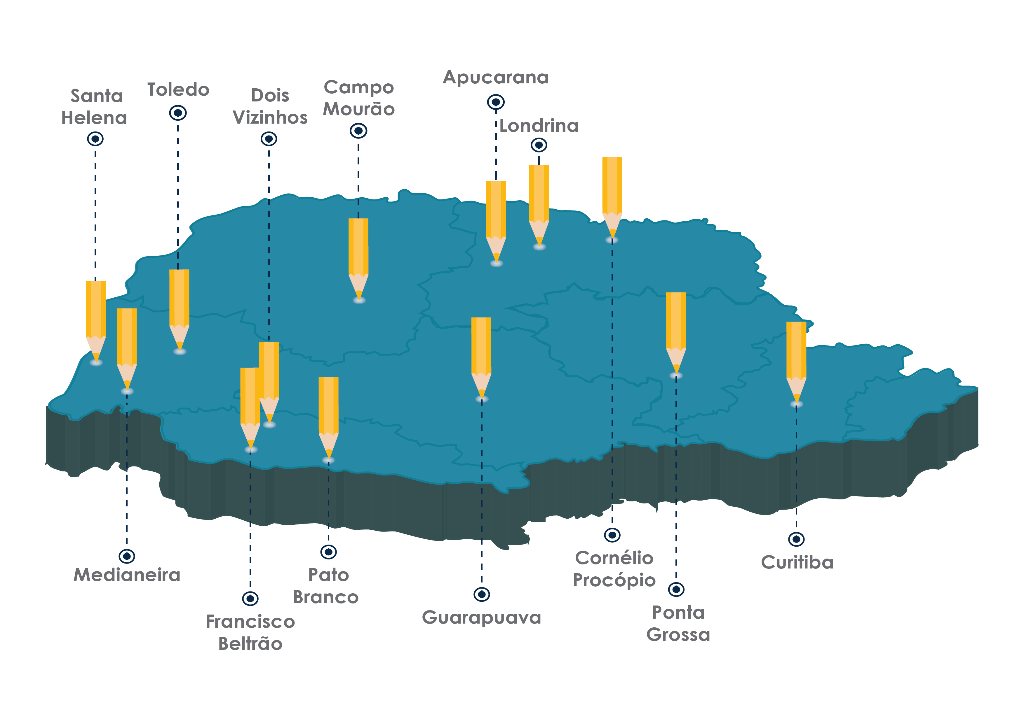
\includegraphics[height = \dimen1]{fig-campi-map}}
			\usebox0%
			\llap{%
				\raisebox{\ht0-\height}{%
					\href{https://www.utfpr.edu.br/campus}{%
						
\includegraphics[height = 10mm]{fig-campi-map-qr-code}%
					}%
				}%
			}
			\SourceOrNote{\textcite{UTFPR2017}}
		\end{figure}
		
		\column{0.5\textwidth-0.5\columnsep}
		
		É possível clicar na Fig.~\ref{fig:flow-experiment-photo} para reproduzir um vídeo dependendo do visualizador de PDF\@.
		
		\begin{figure}[!htb]
			\caption{Experimento de mecânica dos fluidos}%
			\label{fig:flow-experiment-photo}
			\only<presentation>{\dimen1 = 28mm}%% Apresentação: tamanho de figura
			\only<article>{\dimen1 = 48mm}%% Artigo: tamanho de figura
			\movie[showcontrols = true]{%
				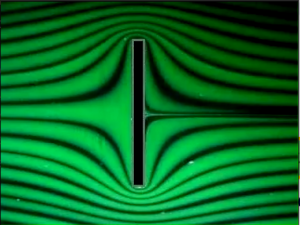
\includegraphics[height = \dimen1]{./Multimedia/flow-experiment-photo}%
			}{./Multimedia/flow-experiment.flv}
			\SourceOrNote{autoria própria (\YearNum)}
		\end{figure}
		
		\begin{exampleblock}{\faExternalLinkSquare*\ Exemplos de atalhos para vídeos (ou outros arquivos)}
			
			\begin{itemize}
				\item[\tiny\faFileVideo] \href{run:./Multimedia/flow-experiment.flv}{Experimento de mecânica dos fluidos (arquivo de vídeo).}
				\item[\tiny\faFileVideo] \href{https://youtu.be/6UlsArvbTeo?si=aU2mbh-XGX3o6nWe}{Escoamento sobre aerofólios (vídeo \ENLang{online}).}
			\end{itemize}
			
		\end{exampleblock}
		
	\end{columns}
	
\end{frame}

\subsection{Gráficos e tabelas}

\begin{frame}
	
	\only<presentation>{\vspace*{-\bigskipamount}}%% Apresentação: espaçamento
	
	\begin{columns}[t]
		
		\column{0.5\textwidth-0.5\columnsep}
		
		A Figura~\ref{fig:t-x}\footnote{Gráfico produzido no ambiente \LaTeX\ \texttt{tikzpicture} do pacote \LaTeX\ \texttt{tikz} a partir do arquivo \texttt{grph-t-x.tex} em \texttt{./Figures/}.} foi inserida usando o ambiente \LaTeX\ \texttt{figure} e numerada automaticamente.
		
		\begin{figure}[!htb]
			\caption{Exemplo de legenda de figura}%
			\label{fig:t-x}
			\only<presentation>{\dimen1 = 36mm}%% Apresentação: tamanho de figura
			\only<article>{\dimen1 = 56mm}%% Artigo: tamanho de figura
			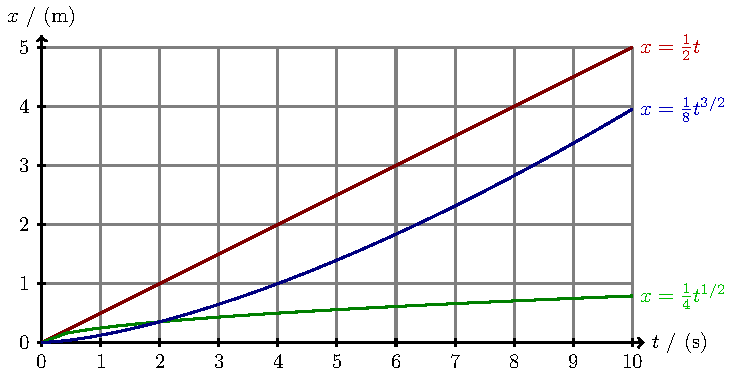
\includegraphics[height = \dimen1]{grph-t-x}
			\SourceOrNote{autoria própria (\YearNum)}
		\end{figure}
		
		\column{0.5\textwidth-0.5\columnsep}
		
		A Tabela~\ref{tab:L-dimensions} foi inserida usando o ambiente \LaTeX\ \texttt{table} e numerada automaticamente.
		
		\begin{table}[!htb]
			\caption{Exemplo de legenda de tabela}%
			\label{tab:L-dimensions}
			\begin{tabularx}{\linewidth}{@{}lYYYY@{}}
				\toprule%
				\multicolumn{1}{@{}c}{\textbf{Caso}} &
				$\MathBF{L / \Unit{(m)}}$            &
				$\MathBF{L^2 / \Unit{(m^2)}}$        &
				$\MathBF{L^3 / \Unit{(m^3)}}$        &
				$\MathBF{L^4 / \Unit{(m^4)}}$        \\ \midrule%
				A & 1 & 1  & 1   & 1   \\
				B & 2 & 4  & 8   & 16  \\
				C & 3 & 9  & 27  & 81  \\
				D & 4 & 16 & 64  & 256 \\
				E & 5 & 25 & 125 & 625 \\ \bottomrule%
				\addlinespace[\belowcaptionskip]
			\end{tabularx}
			\SourceOrNote{autoria própria (\YearNum)}
		\end{table}
		
		\begin{alertblock}{\faInfoCircle\ Ferramentas para gerar ou editar tabelas em \LaTeX}
			
			\begin{itemize}
				\selectlanguage{english}
				\item[\tiny\faTools] \href{https://www.tablesgenerator.com/}{Tables Generator\LinkIcon}.
				\item[\tiny\faTools] \href{https://www.latex-tables.com/}{\LaTeX\ Tables Editor\LinkIcon}.
			\end{itemize}
			
		\end{alertblock}
		
	\end{columns}
	
\end{frame}
